%%%%%%%%%%%%%%%%%%%Sif%%%% file typeinst.tex %%%%%%%%%%%%%%%%%%%%%%%%%
%
% This is the LaTeX source for the instructions to authors using
% the LaTeX document class 'llncs.cls' for contributions to
% the Lecture Notes in Computer Sciences series.
% http://www.springer.com/lncs       Springer Heidelberg 2006/05/04
%
% It may be used as a template for your own input - copy it
% to a new file with a new name and use it as the basis
% for your article.
%
% NB: the document class 'llncs' has its own and detailed documentation, see
% ftp://ftp.springer.de/data/pubftp/pub/tex/latex/llncs/latex2e/llncsdoc.pdf
%
%%%%%%%%%%%%%%%%%%%%%%%%%%%%%%%%%%%%%%%%%%%%%%%%%%%%%%%%%%%%%%%%%%%


\documentclass[runningheads,orivec,a4paper]{llncs}

\usepackage{bbding}
\usepackage{xspace}
\usepackage{wrapfig}
\usepackage{threeparttable}
\usepackage{amssymb,amsmath}
\setcounter{tocdepth}{3}
%\usepackage{verbatim}
\usepackage{graphicx}
\usepackage{subfigure}
\usepackage{amsmath}
\usepackage{bbm}
%\usepackage[ruled,vlined]{algorithm2e}
\usepackage[noend]{algpseudocode}
\usepackage{algorithmicx,algorithm}
\usepackage{url}
\usepackage{color}
%\usepackage{verbatim}
\usepackage{multicol}
\usepackage{lipsum}
\usepackage{xspace}
\newsavebox{\tablebox}
\usepackage{multirow}
%\usepackage{setspace}
%\usepackage{caption}
%\captionsetup[table]{font=small,skip=-4pt} 
%%\usepackage{enumitem}
\usepackage{paralist}
%\usepackage[hang,small,labelfont=,textfont=]{caption}
\usepackage[nodisplayskipstretch]{setspace}
\AtBeginDocument{%
  \addtolength\abovedisplayskip{-0.5\baselineskip}%
  \addtolength\belowdisplayskip{-0.5\baselineskip}%
%  \addtolength\abovedisplayshortskip{-0.5\baselineskip}%
%  \addtolength\belowdisplayshortskip{-0.5\baselineskip}%
}
%\setlength\abovetabcaptionskip{-5pt}
%\setstretch{1}
%\makeatletter
%\renewcommand\normalsize{%
%   \@setfontsize\normalsize\@xpt\@xiipt
%   \abovedisplayskip 1\p@ \@plus2\p@ \@minus5\p@
%   \abovedisplayshortskip \z@ \@plus3\p@
%   \belowdisplayshortskip 6\p@ \@plus3\p@ \@minus3\p@
%   \belowdisplayskip \abovedisplayskip
%   \let\@listi\@listI}
%\makeatother

\let\itemize\compactitem
\let\enditemize\endcompactitem
\let\enumerate\compactenum
\let\endenumerate\endcompactenum
\let\description\compactdesc
\let\enddescription\endcompactdesc
%\usepackage{etoolbox}
%\pltopsep=0pt%\medskipamount
%\plitemsep=0pt
%\plparsep=0pt
%
%%=============added by Rj to reduce space
%\setlength{\parskip}{2pt}
\newcommand{\marginremark}[2]{\annotatedmarginremark{\clubsuit}{$\clubsuit$}{#1}{#2}}
\newcommand{\rjnote}{\color{blue}}
\newcommand{\ccnote}[1]{\marginremark{CH}{#1}}
%\newcommand{\rjnote}[1]{\marginremark{RJ}{#1}}
\def\mathbi#1{\textbf{\em #1}}
% \newcommand{\comment}[1]{}
  \newcommand{\sig}[1]{\textsf{{\small #1}}}
  \newcommand{\nn}{\mathbb{N}}
\newcommand{\bool}{\mathbb{B}}
%\theoremstyle{definition}
%\newtheorem{proposition}{Proposition}
\newtheorem{defi}{Definition}

\begin{document}

%\mainmatter  % start of an individual contribution

% first the title is needed
\title{Contention-aware Task Mapping and Scheduling with Hybrid Search for Heterogeneous NoC-based MPSoCs}

% a short form should be given in case it is too long for the running head
%\titlerunning{A hybrid algorithm for multi-objective mapping and scheduling optimization of MPSoCs}
%\authorrunning{Cheng, Bensalem, Yan, Ruess, Buckl, Knoll}
%% the name(s) of the author(s) follow(s) next
%%
%% NB: Chinese authors should write their first names(s) in front of
%% their surnames. This ensures that the names appear correctly in
%% the running heads and the author index.
%%
%\author{
%Chih-Hong Cheng\inst{1}\inst{2} \and Saddek Bensalem\inst{3} \and Rongjie
%Yan\inst{4} \\ Harald Ruess\inst{1} \and Christian Buckl\inst{1} \and Alois Knoll\inst{2}
%%\and
%%Christian Buckl\inst{5}
%%\and
%%Alois Knoll\inst{1}
%%\and
%%Harald Ruess\inst{4}
%} \institute{
%fortiss GmbH, M\"{u}nchen, Germany   \\
%\and
%Department of Informatics, Technische Universität M\"{u}nchen, M\"{u}nchen, Germany   \\
%\and
%Verimag Laboratory, Grenoble, France\\
%\and State Key Laboratory of Computer Science, ISCAS, Beijing, China\\
%% \url{http://www6.in.tum.de/~chengch/vissbip}
%}

\maketitle
\begin{abstract}


\end{abstract}


%
% The code below should be generated by the tool at
% http://dl.acm.org/ccs.cfm
% Please copy and paste the code instead of the example below. 
%
%\begin{CCSXML}
%<ccs2012>
% <concept>
%  <concept_id>10010520.10010553.10010562</concept_id>
%  <concept_desc>Computer systems organization~Embedded systems</concept_desc>
%  <concept_significance>500</concept_significance>
% </concept>
% <concept>
%  <concept_id>10010520.10010575.10010755</concept_id>
%  <concept_desc>Computer systems organization~Redundancy</concept_desc>
%  <concept_significance>300</concept_significance>
% </concept>
% <concept>
%  <concept_id>10010520.10010553.10010554</concept_id>
%  <concept_desc>Computer systems organization~Robotics</concept_desc>
%  <concept_significance>100</concept_significance>
% </concept>
% <concept>
%  <concept_id>10003033.10003083.10003095</concept_id>
%  <concept_desc>Networks~Network reliability</concept_desc>
%  <concept_significance>100</concept_significance>
% </concept>
%</ccs2012>  
%\end{CCSXML}
%
%\ccsdesc[500]{Computer systems organization~Embedded systems}
%\ccsdesc[300]{Computer systems organization~Redundancy}
%\ccsdesc{Computer systems organization~Robotics}
%\ccsdesc[100]{Networks~Network reliability}


%
% End generated code
%

%
%  Use this command to print the description
%


% We no longer use \terms command
%\terms{Theory}
%\vspace*{-10pt}
%\keywords{task allocation and scheduling; multi-objective optimization; local search; NSGAII framework}
\section{Introduction}\label{se:intro}

The scalable communication architecture makes network-on-chip (NoC) a prevailing solution for the next generation multiprocessor system-on-chips (MPSoCs). 
In the NoC paradigm, an important issue is how to map and schedule tasks of an application to processing elements (PEs), such that the system performance is maximized, while minimizing total energy consumption~\cite{deb2016energy,agyeman2016performance}. Within this architecture, communication is the main concern in the optimization process. To reduce communication consumption, tightly coupled tasks will be closely allocated, which may increase the possibility of communication \textit{contention} for frequent data transfer over same paths.%, or temperature hotspots for keeping some PEs continuously running.  
The increase in contention may incur long latency from network congestion thus leading to high energy consumption and poor system performance. %And the thermal hotspots may incur system reliablility problems. 
Reducing contention requires detailed scheduling and long latency in communication.
Therefore, it is a great challenge for NoC designers to tackle the issues on performance and energy consumption. 

With contention awareness in the design of NoCs, performance and energy consumption optimization need to consider how to map tasks to available PEs and how to schedule tasks on same PEs to avoid contention. 
In this paper, system performance is evaluated by \textit{makespan}, i.e., the scheduling length of the system. And energy consumption encompasses both computation and communication cost. Traditional works mainly focus on communication consumption with respect to the distance and the amount of data between various PEs, and the cost of computation is simplified as the sum of task execution cost on the allocated PEs. Therefore, the design optimization can be reduced to mapping optimization. However, various data transmission activities may require same resources and cause contention, which can lead to the big gap between ideal predication and real performance. 

To optimize performance and energy consumption with the consideration of potential contentions in communication, we construct formulations for mapping and scheduling constraints and objectives to be optimized. Meanwhile, we integrate a problem-specific local search into a  multi-objective evolutionary-based algorithm.  The main contributions of the paper are as follows. First, to reduce spacial contention in mapping, we encode the probability of contention in terms of overlapped paths, and formulate the distribution of contention probability as an objective that can be minimized. Second, to avoid temporal contention in data transmission, we construct the corresponding constraints in scheduling behavior. Third, the energy model encodes the power consumption on links and routers, as well as different modes of PEs. Finally, we construct a hybrid search algorithm, by integrating a local search into a generic algorithm. The algorithm is capable of dealing with large scale applications in approximating better Parent fronts. 
While various design choices exist for NoCs, in this paper, we limit our consideration to 2D mesh networks. 
However, our idea is applicable to other network topologies such as torus and 3D networks.

The rest of the paper is as follows. Section \ref{se:related} discusses related work in the domain static mapping and scheduling. Section \ref{se:concepts} introduces the task model and architecture model. Section \ref{se:model} provides the formulation of the problem. Section \ref{se:alg} presents the details of the algorithm. Experimental results are presented in Section \ref{se:exp}. Section \ref{se:con} concludes the paper.

\section{Related work}\label{se:related}

For embedded systems, energy efficiency is one of critical design issues. Consequently, communication energy minimization is the main concern for the mapping problem of NoCs~\cite{hu2005}. The corresponding cost uses directly or indirectly the average number of packet hops, with bandwidth or latency constraints~\cite{murali2004bandwidth,bhardwaj2009energy,chou2008contention}. 
%Additional to communication cost minimization, thermal balance can also be achieved in mapping optimization~\cite{hung2004thermal}. 
To have a global view of the entire NoC, task mapping and scheduling with the consideration of communication latency is another important problem for the design of NoCs~\cite{yang2014effective,yang2016application}. 
For contention-aware works, considering it in mapping without time information is an over-approximation of contentions~\cite{chou2008contention}. Though the work in \cite{yang2016application} considers contention in scheduling, it introduces latency to avoid contention and mainly focuses on makespan minimization. He et al. estimate traffic congestions by using heuristics~\cite{he2012unism}. Han et al. consider contention and energy-aware in mapping and scheduling, with pre-defined priorities for tasks and data transmissions~\cite{han2015contention}. 
To evaluate performance globally, we introduce contention reduction in both mapping and scheduling, and both performance and energy consumption can be optimized at the same time. 
%Meanwhile, we use overlapped area of two paths to quantify the probability of contention, which allows us to trade off between contentoin minimization and the capacability limitation of PEs.
 
Various algorithms exist for mapping optimization, such as tabu search~\cite{tino2011multi}, branch-and-bound~\cite{hu2003energy}, binary particle swarm optimization~\cite{lei2010energy}, and diagonal map~\cite{agrawal2010efficient}. Similar to the solutions for MPSoCs, genetic algorithms~\cite{nedjah2014application}, simulated annealing algorithm~\cite{chai2014list}, mixed integer linear programming (MILP)~\cite{yang2016application} have also used to solve the mapping and scheduling problems. 
An ILP formulation has been proposed for contention aware application mapping in tile based NoC to reduce inter-tile network contention\cite{chou2008contention}. 
%To minimize average communication delay and satisfy bandwidth constraints, Murali and De Micheli use minimum path routing in mapping optimization~\cite{murali2004bandwidth}. 
Huang et al. propose a simulated annealing algorithm with timing adjustment heuristic is proposed to minimize energy consumption \cite{huang2011energy}. 
%In the work of \cite{zang2015energy}, a genetic algorithm is applied to minimize both energy and hotspot temperature. 
These works only consider mapping issues for NoCs. 
The work in \cite{bolanos2013uml} employs population based incremental learning algorithm for mapping and scheduling optimiztation. He et al. introduce a unified model in mixed integer linear programming, for task mapping and scheduling~\cite{he2012unism}. 
%A partitioned earliest deadline first strategy is applied in an allocation algorithm for maximizing resource untilzation while minimizing average end-to-end worst case response time~\cite{ali2013critical}. 
An ILP formulation encoding fine-grain communication optimization is proposed in \cite{yang2016application}. And a heuristic algorithm is designed for application mapping and scheduling. To optimize the objectives in our constraint formulation, we put forward a hybrid search algorithm for both performance and energy optimization.
 Therefore, from the aspect of our formulation and the algorithm, the techniques discussed in the paper are different from existing works.


\section{Preliminaries}\label{se:concepts}
We consider applications represented using task graphs (TGs). A task graph is a directed acyclic graph (DAG).
\begin{defi}[Task Graph]
A task graph is a directed acyclic graph (DAG) with $G=\langle T,E\rangle$, where $T$ is a finite set of tasks, with $\delta: T\rightarrow \nn$ to indicate the amount of work to be dealt with on each task, and $E\subseteq T\times T$ is a set of precedence relations with $c: E\rightarrow \nn$ to indicate the amount of data transferred between each pair of tasks.
\end{defi} 
Each vertex may have a relative deadline, specifying the latest tolerable finishing time w.r.t. the start time of the first task in a period. %And a latest response time may also exist between various tasks. 
The model shown in Figure~\ref{fig:taskgraph}(a) is a task graph with 4 tasks and 5 dependency relations.  
\begin{figure}
\centering
 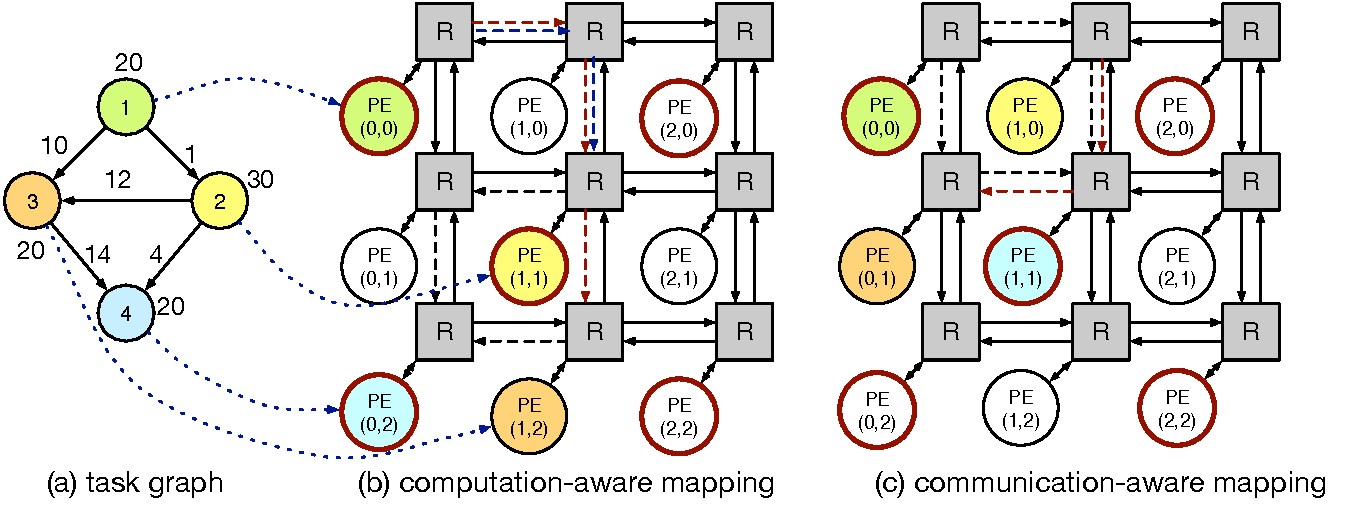
\includegraphics[width=0.85\columnwidth]{figures/running_example}% \vspace{-4.5mm}
  \caption{A running example.}
 \label{fig:taskgraph}
% \vspace{-3mm}
 \end{figure}
 
The target hardware is a 2D mesh NoC-based heterogeneous MPSoCs, as illustrated in Figure \ref{fig:taskgraph}(b). Each PE in the model is connected to a \textit{router}. And routers are connected with each other through bidirectional \textit{links}. Data transmission through the NoC is in the form of packets. If two consequential tasks are mapped to the same PE, data can be directly read without routing. Within this topology, the location of each PE 
can be determined by a pair of coordinates $(x_i,y_i)$. And the distance between any two PEs $p_i$ and $p_j$ is the Manhattan distance:
\begin{equation}
D_{ij}=abs(x_i-x_j)+abs(y_i-y_j)
\end{equation}
%XY-routing is assumed in this paper. 
Figure~\ref{fig:taskgraph}(b) shows an  example with 3$\times$3 nodes of two different types of processors, where the speed of processors with red cycles is two times faster than others. The communication is assumed to have cost 1 per unit payload per link.

We present two kinds of mappings for the model in Figure~\ref{fig:taskgraph}(a), where one utilizes faster processors and the other minimizes communication paths. With the mapping in Figure~\ref{fig:taskgraph}(b), the cost of computation is 55, and the cost of communication is 66, if we only consider the cost in links, and ignore the latency caused by contention during communication. For the case in Figure~\ref{fig:taskgraph}(c), the cost of computation is 70, and the cost of communication is 53. The first mapping have a contention between communications from $p_{00}$ to $p_{11}$ and from $p_{00}$ to $p_{12}$. However, the caused delay is only 1. Therefore, it is hard to choose without detailed performance and energy consumption information. 




\section{Constraint formulation}\label{se:model}
Compared with other formulations, the features of our model are as follows.
First, we evaluate the allocation and scheduling strategy for a certain number of iterations, instead of once execution of every task. This allows a more accurate system evaluation. Second, additional to the deadline for every task, we put forward the concept of latest response time between two tasks, to meet the requirements of time-critical systems. Third, we consider fine-grained communication in the case of contentions. Finally, besides energy consumption and performance optimization, we also consider to minimize the probability of contention caused by communication from different resources in a communication network, which is evaluated by the overlapped area between two communication paths. 

%The hardware architecture considered here is a general framework, e.g., MPSoCs or NoCs. 
%%The performance is still evaluated with makespan, which is the duration of the executing of an application. 
%We assume that communication does not occupy computation resources, except for setup efforts.
%The channel for communication may consist of multiple links and nodes. Multiple data transfer may happen at the same time, or cannot overlapped, which is decided by the architecture.

First, we introduce the variables and constants used in our formulation in Table \ref{tab:var}, to present the constraints in allocating and scheduling issues.
\begin{table}[t]\caption{Constants and Variables \label{tab:var}}
\centering\small
\begin{tabular}{l l}\hline
Item & explanation\\\hline$bw$ & the bandwidth of a link \\
$\tau$& the time  of transferring a unit with unit distance\\
$\tau'$& the time  of transferring a unit through a node\\
$\epsilon$ & the energy of transferring a unit with unit distance\\
$\epsilon'$ & the energy of transferring a unit through a node\\
$a_i$ & the amount of computation for task $t_i$ \\
$c_{ij}$ & the amount of data to be transferred from task $t_i$ to $t_j$\\
%$q_i$ & the required size for data storage of $t_i$\\ 
$dl_{ij}$ & maximal time allowed between executing task $t_i$ and $t_j$\\
$\rho_k$ & processing speed of  $p_k$\\
$\omega_k$  & the memory limit for $p_k$ \\
%$\eta$ & the cost of communication setup \\
$\gamma_{{i_1}{j_1}{i_2}{j_2}}$ & the number of shared transmission path exists from $p_{i_1}$ to $p_{j_1}$ and from $p_{i_2}$ to $p_{j_2}$\\
$\xi$ & the time bound for simultaneous communication \\
$N$ & the number of iterations for all the tasks\\\hline
$m_{ik}$ & task $t_i$ is mapped to  $p_k$ \\
$n_{ij}$ & task $t_j$ is executed next to $t_i$ on the same processor\\
$s_i$  & the start time of executing task $t_i$ \\
$f_i$& the end time of executing task $t_i$ \\
$se_{ij}$ & the start time of data transfer from $t_i$ to $t_j$\\
$fe_{ij}$ & the finish time of data transfer from $t_i$ to $t_j$\\
%$ss_i$  & the start time of data transfer for task $t_i$ \\
%$fs_i$& the end time of data transfer for task $t_i$ \\
%$sr_i$  & the start time of receiving data for task $t_i$ \\
%$fr_i$& the end time of receiving data for task $t_i$ \\
$d_{ij}$ & task $t_j$ depends on the output of $t_i$\\
$o_{ij}$ & task $t_i$ needs to send data to its successor\\
$D_{ij}$ & distance between $p_i$ and $p_j$\\
$P_{ij}$ & the contention probability of data transfer from two tasks\\
\hline
\end{tabular}
\end{table}

%\begin{table}[htp]\caption{Constants\label{tab:con}}
%\centering
%\begin{tabular}{ll}\hline
%Item & explanation\\\hline
%$bw$ & the bandwidth of a link \\
%$\tau$& the time  of transferring a unit with unit distance\\
%$\tau'$& the time  of transferring a unit through a node\\
%$\epsilon$ & the energy of transferring a unit with unit distance\\
%$\epsilon'$ & the energy of transferring a unit through a node\\
%$a_i$ & the amount of computation for task $t_i$ \\
%$c_{ij}$ & the amount of data to be transferred from task $t_i$ to $t_j$\\
%%$q_i$ & the required size for data storage of $t_i$\\ 
%$dl_{ij}$ & maximal time allowed between executing task $t_i$ and $t_j$\\
%$\rho_k$ & processing speed of  $p_k$\\
%$\omega_k$  & the memory limit for $p_k$ \\
%%$\eta$ & the cost of communication setup \\
%$\gamma_{{i_1}{j_1}{i_2}{j_2}}$ & the number of shared transmission path exists from $p_{i_1}$ to $p_{j_1}$ and from $p_{i_2}$ to $p_{j_2}$\\
%$\xi$ & the time bound for simultaneous communication \\
%$N$ & the number of iterations for all the tasks\\
%\hline
%\end{tabular}
%\end{table}

In Table \ref{tab:con} can be computed according to the positions of processors. Given processors $p_{i_1}$, $p_{j_1}$, $p_{i_2}$ and $p_{j_2}$, let $(x_i,y_i)$ be the location of $p_i$. We have 
\begin{small}
 $$oX'=(x_{j1}-x_{i_1})+(x_{j2}-x_{i_2})-(max\{x_{j_1},x_{j_2}\}-min\{x_{i_1},x_{i_2}\})$$
 $$oY'=(y_{j1}-y_{i_1})+(y_{j2}-y_{i_2})-(max\{y_{j_1},y_{j_2}\}-min\{y_{i_1},y_{i_2}\}).$$
\end{small}
Let $oX=max\{oX',0\}$, and $oY=max\{oY',0\}$. We have $\gamma_{{i_1}{j_1}{i_2}{j_2}}=oX+oY$.  

\subsection{Constraints}
The constraints can be divided into two types: static mapping and dynamic behaviors. For behavior constraints, they consist of computation and communication behaviors. 

\subsubsection{Static constraints}
\begin{equation}\label{eq:map}
\sum^{|P|}_{k=1} m_{ik} =1
\end{equation}
\begin{equation}\label{eq:cap}
\sum^{|T|}_{i=1} m_{ik} \cdot q_i \leq \omega_k
\end{equation}
\begin{equation}\label{eq:neighbor}
n_{ij} + n_{ji} \leq 1 \wedge (n_{ij}\wedge n_{jl} \rightarrow \neg n_{il}), ~~n_{ij}\leq m_{ik}\cdot m_{jk'}
\end{equation}
\begin{equation}\label{eq:aux}
d_{ij}\wedge m_{ik}\wedge m_{jk'}\wedge (k\neq k') \rightarrow o_{ij}, ~~o_{ij}\rightarrow d_{ij}
\end{equation}
Constraint \ref{eq:map} requires that one task can only be mapped to one processor.
Constraint \ref{eq:cap} specifies that the capacity of a processor cannot be violated.
Constraint \ref{eq:neighbor} explains that the next-door execution relation is not transitive and reflexive.
Constraint \ref{eq:aux} reasons the case with communication cost.

\subsection{Dynamic behaviors}
First, we present precedence relation for computation and communication.
\begin{equation}\label{eq:response}
s^v_j-s^u_i\leq dl_{ij}
\end{equation}
\begin{equation}\label{eq:datar}
\sum^{|T|}_{j=1}d_{ji}>0 \rightarrow fe^u_{ji} \leq s^u_i
\end{equation}
\begin{equation}\label{eq:datas}
f^u_i\leq se^u_{ij}
\end{equation}
\begin{equation}\label{eq:next}
n_{ij} \rightarrow f^u_i \leq s^v_j \textrm{, for~} u\leq v
\end{equation}
\begin{equation}\label{eq:period}
m_{ik}\wedge m_{jk}  \rightarrow f^u_j \leq s^v_i \textrm{, for~} u<v
\end{equation}
Constraint \ref{eq:response} specifies that  the response time between certain tasks should less than the defined limitation.
Constraint \ref{eq:datar} requires that the start of executing $t_i$ should wait for data being transferred, except for the one without any predecessor.
Constraint \ref{eq:datas} specifies that the start of data transfer has to wait for the finish of task execution.
Constraint \ref{eq:next} requires that for two tasks scheduled next to each other in the same processor, the start of the latter should wait for the finish of the former, where $u\leq v$.
Constraint \ref{eq:period} explains that  the execution of task in later iteration $v$ should not be earlier than any other tasks executed on the same processor in an earlier iteration $u$, where $u<v$.

Next, we present constraints to avoid overlapped computation and communication. 

\begin{equation}\label{eq:overlap}
m_{ik}\wedge m_{jk} \rightarrow s^u_j\geq f^u_i \vee s^u_i\geq  f^u_j
\end{equation}
%\begin{equation}\label{eq:commlap}
%m_{ik}\wedge m_{lk}\rightarrow se^u_{ij}\geq fe^u_{lr} \vee se^u_{lr}\geq  fe^u_{ij}
%\end{equation}
\begin{equation}\label{eq:samesource}
\gamma_{{i}{j}{i}{r}} \rightarrow se^u_{ij}-se^u_{ir}\geq \xi
\end{equation}
\begin{equation}\label{eq:linklap}
\gamma_{{i}{j}{l}{r}}\wedge abs(f_{i}-f_{l})\leq \xi \rightarrow se^u_{ij}\geq fe^u_{lr} \vee se^u_{lr}\geq  fe^u_{ij}
\end{equation}

Constraint \ref{eq:overlap} specifies that two tasks executed on the same processor cannot be overlapped. 
%Constraint \ref{eq:commlap} explains  two communications from the same source cannot overlap.
Constraint \ref{eq:samesource} says that data transfer sharing same links from the same source cannot be triggered simultaneously. 
Constraint \ref{eq:linklap} says that two communication with shared resource cannot overlap, if their tasks finish execution almost at the same time. This constraint aims to allow the following case shown in Figure~\ref{fig:overlap}. A short communication path from $p_2$ to $p_3$ is overlapped by a long communication path from $p_0$ to $p_3$. But the communication of the short path can be finished before the long transmission arrives the shared path. 
%\item before receiving, a successor has wait for the finish of data transfer from its predecessor 
%\begin{equation}\label{eq:dependency}
%d_{ij}\wedge m_{ik}\wedge m_{jk'}\rightarrow fs^u_i \leq sr^u_j
%\end{equation}
\begin{figure}[h]
\centering
 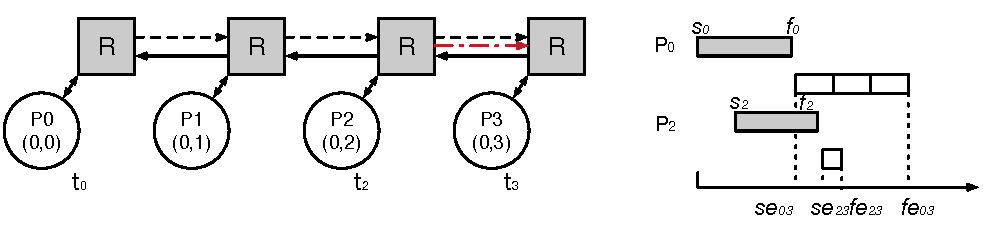
\includegraphics[width=0.85\columnwidth]{figures/overlap.pdf}% \vspace{-4.5mm}
  \caption{An example with communication overlap.}
 \label{fig:overlap}
% \vspace{-3mm}
 \end{figure}

Next we present quantitative relation for the variables on computation and communication.

\begin{equation}\label{eq:comp}
f^u_i = s^u_i + a_i/(\sum^{|P|}_{k=1} m_{ik}\cdot \rho_k)
\end{equation}
\begin{equation}\label{eq:comm}
fe^u_{ij} \geq se^u_{ij} +  o_{ij}\cdot(c_{ij} \cdot\tau\cdot  D_{ij}/bw+\tau'\cdot (D_{ij}+1))
\end{equation}
Constraint \ref{eq:comp} presents task execution relation.
Constraint \ref{eq:comm} shows that the finish of a data transfer considers the distance of the destination%two processors $p_k$ and $p_{k'}$
where $D_{ij}$ is the distance from the located processor of $t_i$ to the target processor. 

%\noindent\textbf{Discussion.} 
%The constraints listed above are flexible. For example, Constraint \ref{eq:period} can be relaxed such that a task can be executed several times before the next scheduled.

%As these constraints are for a general framework, we can adjust it according to specific architectures, especially for communication issues. For example, if the architecture allows multiple communication simultaneously,  Equation \ref{eq:commlap} can be relaxed.
%
%The communication link for different architectures may be quite different. For an MPSoC with buses connected to processors, there is not intermediate node or link between two processors. However, for an NoC, the situation is quite different, where the communication between two processors is fulfilled through links for transmission and switches for router.
%%Compared with general MPSoCs, the communication cost in NoC is more complex to evaluate, which consider the number of links and switches between two communicated processors.
%
%We consider 2D-mesh NoC, where the effort for communication can be computed according to the distance between two processors $p_i$ and $p_j$, where $(x_i,y_i)$ is the location of $p_i$\cite{huang2011energy}:
%\begin{equation}\label{eq:dis}
%D_{ij}=abs(x_i-x_j)+abs(y_i-y_j)
%\end{equation}

\subsection{Optimization objectives}

With the defined variables, the makespan of  executing an application within $N$ iterations is 
\begin{equation}\label{eq:makespan}
{\cal{M}}=max\{f^N_i\}
\end{equation}
However, energy consumption includes cost for computation $E_p$ and communication $E_m$. For computation, we distinguish different status in a processor and accumulate the total cost. For communication, we consider the cost for routing and data transfer. In a NoC network, the number of available processors may be larger than that of tasks. We use $P'=\{p_k\;| \sum^{|T|}_{i=1} m_{ik}>0\}$ to denote the set of occupied processors. 

A processor may switch between dynamic, static and sleep modes, to save energy consumption. If the idle time is less than $t_{o}$, the processor will not switch into sleep mode. Otherwise, a time penalty $t_\Delta$  for switching into and out of sleep is considered, together with an energy penalty $\epsilon_\Delta$.
%We ignore power leakage, for we take computation load balance as one of optimization goals, which can keep the chip in a relative steady temperature. 
The execution duration of every iteration in a processor may be different, thus the cost should differ. Let $t_h$ be head of scheduled task in a processor $p_k$ in every iteration, where the constraint  $\sum^{|T|}_{j=1} m_{jk}-1=\sum^{|T|}_{j=1} q_{k_{hj}}$ holds. The duration ${\mathcal{D}}^u_{k}$ for processor $p_k$ in iteration $u$ is
\begin{equation}\label{eq:duration}
{\mathcal{D}}^u_{k} =\left\{
\begin{array}{ll}
\tau^{u+1}_h -\tau^u_h & u<N\\
{\mathcal{M}} - \tau^N_h & u=N
\end{array}
\right.
\end{equation}
Let $t_l$ be the tail of scheduled task in $p_k$, with $\sum^{|T|}_{i=1} q_{k_{li}}+1=m_{lk}$.
Then the spare time ${\mathcal{S}}^u_{k_{ij}} $for a processor $p_k$ executing two successive tasks $t_i$ and $t_j$ in iteration $u$ can be computed as follows:
\begin{equation}\label{eq:spare}
{\mathcal{S}}^u_{k_{ij}} =\left\{
\begin{array}{ll}
0 & \gamma_{k_{ij}}=0\wedge i\neq l\\
\tau^u_j-e^u_i & \gamma_{k_{ij}}=1 \wedge i\neq l\\
{\mathcal{D}}^u_k-e^u_i & i=l
\end{array}\right.
\end{equation}

Let ${\mathcal{P}}_{d_k}$, ${\mathcal{P}}_{i_k}$ and ${\mathcal{P}}_{s_k}$ be the rate of dynamic, static (idle) and sleep power consumption of processor $p_k$, respectively. The costs for dynamic ($E_d$), static and sleep ($E_{is}$) are calculated as follows:
 \begin{equation}
E_d = N\cdot \sum^{|P'|}_{k=1}({\mathcal{P}}_{d_k}\cdot \sum^{|T|}_{i=1}  \theta_i \cdot m_{ik})
\end{equation}%\vspace{-10pt}
\begin{equation}\label{eq:ei}
E_{is} =\sum^N_{u=1}\sum^{|P'|}_{k=1}\sum^{|T|}_{i,j=1}\left\{
\begin{array}{ll}
{\mathcal{P}}_{s_k}\!\!\cdot ({\mathcal{S}}^u_{k_{ij}}-t_\Delta) + \epsilon_\Delta & {\mathcal{S}}^u_{k_{ij}} \!\!\geq t_{o} \\
 {\mathcal{P}}_{i_k}\!\!\cdot {\mathcal{S}}^u_{k_{ij}} &0 \leq {\mathcal{S}}^u_{k_{ij}}\!\! <t_{o} %\\
 %0 & ~~{\mathcal{S}}^u_{k_{ij}}=0
\end{array}
\right.
	%E_i= \sum^{|P|}_{k=1} (Ri_k \cdot ({\cal{M}}- N\cdot \sum^{|T|}_{i=1}  \theta_i \cdot m_{ik} ) )
\end{equation}%\vspace{-14pt}




The energy cost for communication is evaluated according to the amount of data and the distance of the transmission. 
\begin{equation}\label{eq:ecomm}
E_m = N\cdot  \sum^{|P'|}_{k,k'=1} \sum^{|T|}_{i,j=1} c_{ij}\cdot o_{ij}\cdot m_{ik}\cdot m_{jk'}\cdot (\epsilon\cdot  D_{kk'}+ \epsilon'\cdot (D_{kk'}+1))
\end{equation}

Addition to the energy and makespan optimization, we also expect that the probability of communication contention is reduced. As data transfer occurs in the end of task execution, we consider the potential contention when two tasks at various processors finish execution almost simultaneously (their difference is less than a limited time bound. The probability is evaluated according to the overlapped path between two communication paths in a communication network. Suppose two paths are from processor $i_1$ to $j_1$, and $i_2$ to $j_2$ respectively.  
%Let $oX$ and $oY$ be the overlapped width and length of the two paths. That is
%\begin{small}
% $$oX=(x_{j1}-x_{i_1})+(x_{j2}-x_{i_2})-(max\{x_{j_1},x_{j_2}\}-min\{x_{i_1},x_{i_2}\})$$
% $$oY=(y_{j1}-y_{i_1})+(y_{j2}-y_{i_2})-(max\{y_{j_1},y_{j_2}\}-min\{y_{i_1},y_{i_2}\}).$$
%\end{small}
% If $oX\leq 0$ or $oY\leq 0$, there is no contention. Therefore, we have $oX=max\{oX,0\}$, and $oY=max\{oY,0\}$. 
% Let the areas of the two paths be $S_1=abs((x_{i_1}-x_{j_1})\cdot (y_{i_1}-y_{j_1}))$ and  $S_2=abs((x_{i_2}-x_{j_2})\cdot (y_{i_2}-y_{j_2}))$ respectively. 
The contention probability of two paths is 
\begin{equation}
%p_c({i_1},{j_1},{i_2},{j_2})=oX\cdot oY/(S_1+S_2)
p_c({i_1},{j_1},{i_2},{j_2})=(oX+ oY)/(D_{{i_1}{j_1}}\cdot D_{{i_2}{j_2}})
\end{equation}

For any two tasks $t_{i_1}$ and $t_{i_2}$, let ${\mathcal{T}_{i}}$ be the set of successors of task $t_i$. Then the measure of contention of communication is 
\begin{equation}\label{eq:submeasure}
P_{{i_1}{i_2}}=\sum_{j_1\in {\mathcal{T}_{i_1}}, j_2 \in {\mathcal{T}_{i_2}}}(abs(f^u_{i_1} -f^v_{i_2})\leq \xi)\cdot o_{{i_1}{j_1}}\cdot o_{{i_2}{j_2}}\cdot p_c(k_{i_1},k_{j_1},k_{i_2},k_{j_2})
\end{equation}
%However, data transmission is fulfilled by bus in an MPSoC, we have 
%\begin{equation}
%P_{{i_1}{i_2}=}(abs(f^u_{i_1} -f^v_{i_2})\leq \xi)
%\end{equation}
According Equation \ref{eq:submeasure}, the measure for a mapping and scheduling strategy is 
\begin{equation}
P_c=\sum^{|T|}_{i,j=1} P_{ij}
\end{equation}
We apply the average contention probability to evaluate the quality of the allocation strategy, which is denoted by
\begin{equation}
\bar{P_c}=\sum^{|T|}_{i,j=1}abs(P_{ij}-P_c/(|T|\cdot N))
\end{equation} 
Based on the discussion above, we can have three objectives to be optimized: makespan, total amount of energy cost, and contention:
\begin{equation}\label{eq:makespan}
minimize({\cal{M}})
\end{equation}
\begin{equation}\label{eq:energy}
minimize(E_{pd} +E_{is}+ E_m)
\end{equation}
\begin{equation}\label{eq:contention}
minimize(\bar{P_c})
\end{equation}
\noindent\textbf{Discussion.} 
Constraint \ref{eq:linklap} and Objective \ref{eq:contention} are complementary. Constraint \ref{eq:linklap} considers the temporal relation of contention, and separates the potential overlapped communication mandatory to avoid contention. Objective \ref{eq:contention} focus on spatial contention and tries to minimize the overlapped communication paths. 
%For an NoC, workload balance is not the main concern, for the number of available processors may be greater than that of tasks.



%\vspace{-5pt}

\section{The hybrid search algorithm}\label{se:alg}
As a result of the complexity of the multi-objective optimization and the enormity of searching exploration, some efficient strategies should be proposed to differentiate non-dominated solutions and enhance the selection pressure towards the pareto front. Accordingly, we have integrated a pareto local search method into the NSGAII framework together with objective-related heuristic extensions, aiming to tackle the mapping and scheduling on NoC paradigm. This approach consists of three stages of optimization based on the characteristic of the model mentioned above. The first stage is a task-grouping process, which aims to cluster the tasks with more dependence into one core. It is obvious that if more dependent tasks are gathered in the same core, less communication will occur, without other factors considered in this stage. Then, due to the heterogeneous architecture and communication  constraints, a core-tile mapping stage is needed to optimize the makespan and average contention probability. An inadaptable mapping will cause more congestion or remote transmission distance. At last, we are looking for a better sequence scheduling in each tile so as to minimize the makespan and satisfy the response time requirement between certain tasks. It should be noted that these three stages are initialized in a heuristic way in order, but are evolved in the evolution process as a whole. The optimization of each stage can be regarded as a multi-objective problem, so the incorporation of these three difficult problems make the mapping and scheduling more intractable. Also, three realistic objectives are considered, which increases the difficulty of this issue to a great extent. Detailed information about the algorithm is discussed in the following subsections.
\subsection{Encoding}
Before introducing the evolutionary algorithm, the representation of chromosome, which indicates the form of solution to the problem, is given. As is discussed in section 3, the location of each PE can be determined by a pair of coordinates $(x_i,y_i)$ within 2D mesh topology, which is troublesome for genetic operators. Each operative tile $p_k$ in the NoC has an associated gene which encodes the identifier of the core mapped in the tile. Thus, for a $n*m$ Noc, the chromosome encoding for the mapping and scheduling problem is shown in Fig.\ref{fig:encoding}. Every chromosome contains a set of mapped tasks, and the scheduled execution sequence for the allocated processors, which varies from conventional encoding for mapping optimization. Therefore, we need extra pointers to separate the genes for various processors. Moreover, three tips should be considered.
\begin{enumerate}[(1)]
\item $p_k \in P'$ is guaranteed, which means only the occupied processors are taken into consideration in the chromosome. 
\item $p_k$ can be translated into the location of 2-dimension coordinates $(x_i,y_i)$ in such a way: $x_i=k/m, y_i=k$ \textit{mod} $m$.
\item The index of $p_k$ may not be continuous but should be in ascending order for the reason of idle tiles. As is shown in Fig.\ref{fig:encoding}, $p_2$ does not appear because no tasks are assigned on tile $(0,2)$. However, if there are tasks migrating to tile $(0,2)$ during evolution process, $p_2$ should be added into the position between $p_1$ and $p_3$ in order to map the tile $(0,2)$.
\end{enumerate} 
Next, we will discuss some primary components of the algorithm in detail and provide the whole framework.
\begin{figure}[h]
\centering%\vspace{-8pt}
 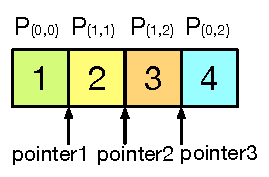
\includegraphics[width=0.2\columnwidth]{figures/encodingy.pdf}%\vspace{-10pt}
  \caption{Chromosome encoding}
 \label{fig:encoding}
 %\vspace{-5mm}
 \end{figure}
%\vspace{-5pt}
\subsection{Initialization}
The idea behind the proposed initialization is to blend some priori knowledge or heuristic information into the pure random construction adopted by general research, for the reason that the exploration space for three-objective is fairly wide. A diversified population could provide a greater chance to find the optimal, yet would result in slow convergence. While an intensified population could converge fast, yet would make the algorithm trap into local optimum. By this token, some candidate solutions would be generated randomly to cover a more comprehensive solution domain, while a few constructive solutions are also needed to store problem-heuristic information for a faster convergence. So given the three stages of optimization, the initialization process could be divided into two steps, and the scheduling optimization is mixed together with grouping and mapping to reduce the complexity of the method.

We adopt different strategies against various situation of the task graph. Most techniques deflect to the reduction of communication cost, as communication is the major concern in the optimization process. The first heuristic solution for grouping is generated by following steps, which takes makespan and communication into consideration. 
\begin{enumerate}[(1)]
\item If the task graph is disconnected, the number of groups we classify is equal to the amount of connected components, and each connected component is regarded as a group. In this way, no packets will be transmitted in the network.
\item Conversely, if there are no disconnected graphs in the task graph, a distribution of parallel tasks is recommended to be executed simultaneously. For each task $t$, in-degree $In(t)$ is calculated according to the dependency relation of tasks. For the task whose $In(t)$ is zero, it is pushed into the execution sequence, and if there are other tasks whose $In(t)$ is zero, they are pushed into the execution sequence and locked. Every time an unlocked task is popped and assigned to the current group. Then, the in-degrees of its successors decrease by 1. When no tasks are allowed to allocate, unlock one task in the execution sequence and divide it into a new group. Loop continues until all the tasks are assigned. The sequence of popped tasks also represents a scheduling plan to the problem, because every task is guaranteed to be executed after its dependent tasks.
\item It should be noted that too many parallel tasks will cause an exceeding number of groups comparing with limited PEs. Thus, some groups should be mapped into the same PE. The fulfilment is inspired by the fact that the processors with minor tasks will be idle for a long time, which is a waste of energy consumption. So, the groups are ranked in descending order by the computation time, and we try to merge the last two groups into a new one every time until the number of groups meets the quantitative requirement. The rule of combination follows an insertion-in-turn operator, meaning that the element selected to be inserted into the new group from one group is followed by the task from another, which keeps the sequence of tasks in the original group unchanged. For the tasks whose execution sequence are inadequate within the group, delay them until their dependent tasks having been performed.
\end{enumerate} 

The output of grouping stage is an input of mapping process, including a set of groups.

In order to accelerate the convergence of mapping, an easy implementing called Spiral algorithm is adopted as~\cite{mehran2007spiral} does. Different from the original task searching, a group searching is proposed to reduce communication cost ulteriorly. The placement of a group is searched in a spiral path from centre to the boundary of the network architecture. It tries to place the communicating groups close to each other, decreasing the transmission path between two PEs. Furthermore, the characteristic of spiral architecture makes communicating groups locate on different directions in order to lower the probability of potential contention. With the mapping rules above, the transmission cost between each group and the total cost of one group is calculated respectively. Afterwards, the most costly group is assigned to the center and next to it is the group with the highest transmission cost to communicate. Break ties randomly if there exist more than one feasible groups. 
The initial solution with heuristic information is hereby generated and other solutions are produced in a random mode to cover a wider searching space. In this way, we can obtain an initial population with a balance between the diversified population and the convergence.
Then the initial population will be divided into several sub-populations by the non-dominated sorting strategy in NSGAII, each of which is sorted according to the crowding distance to ensure a wider distribution.
\subsection{Genetic Process}
In this process, we propose an uniform crossover and a split (or merge) based mutation operator in the genetic procedure, to improve the feasibility and diversity of solutions. 

The crossover operator performs a random selection of two parents from the dynamic elitist population and the evolution population. Then each task in the offspring inherits the position in one of its parents randomly. So, the positions of every task in the parents are recorded. The uniform crossover can help avoid the case that a task is assigned to different processors.

The mutation operator focuses on the conversion of task mapping for the purpose that subsequent local search is applied based on the fixed mapping, which is easier to trap into the local optimum given a constant mapping. To be specific, each individual receives a mutation probability, neither too small nor too large. A small probability will cause a long time stagnation on evolution, while a large one will lead to an insufficient search for the existing structure. For mutation, an occupied probability $P_o$ is calculated as $P_o=|P'|/|P|$, and a split perturbation will be adapted on a probability of $P_o$, together with a merge perturbation executed on a probability of ($1-P_o$). In this way, it is possible to adjust the number of running processors dynamically according to the occupied status. More processors are likely to be allocated if tasks have gathered into a few processors, and the combination of processors with low utilization is preferred if the distribution of tasks is scattered. In a split operator, the most time-consuming processor is supposed to decompose into two light processors, each of which shares half of the computation load. The new generated processors are mapped into the first two available PEs in terms of the spiral rule. As for the merge operator, it is performed the same as initial procedure does except that the merge stage is conducted only once and the incorporative processor is mapped into the first available PE according to the spiral rule. 
\subsection{Pareto local search}
In the $\epsilon$-MOHA algorithm, we use a pareto local search (Alg\ref{alg3}) to enhance the intensive searching capacity. The procedure consists of a repair step for infeasible solutions, an insert-based
neighbourhood comparison and generation step.

A repair operator on the infeasible solutions is needed to spare the resource (Alg\ref{alg3}.line 2). The main idea of \textit{repair} operator is to repeatedly check the feasibility of executing tasks and ensure that each task begins to execute later than all its dependent tasks.

Another important factor in the Pareto local search procedure is the neighborhood structure. Given a candidate solution \textit{S} and two tasks $t$ and $t'$, if we only insert the position of the task $t$ into the head of task $t'$ and fix the positions of other tasks, we can obtain a neighbor solution of \textit{S}. We then use \textit{neighbor($S_t$)} to denote the set of neighbors of \textit{S} by inserting $t$ into other positions. In the main Pareto local search loop (Alg\ref{alg3}.line 3-10), the algorithm randomly selects a task $t$ of solution $S$ (Alg\ref{alg3}.line 4) and tries to find a solution that can $\epsilon$-dominate $S$ from its neighborhood space (Alg\ref{alg3}.line 5). Specifically, if \textit{neighbor($S_t$)} is better than \textit{S} based on Pareto optimal evaluation, it will replace \textit{S} for further exploitation and $iter$ is set to 1 to look for a better neighorhood than the current. Meanwhile, the elitist population $S_E$ is updated (Alg\ref{alg3}.line 6-8). Otherwise, another task will be selected and $iter$ will be increased by 1 (Alg\ref{alg3}.line 10). This process continues until $iter$ reaches the maximum limit.

\begin{algorithm}\scriptsize
\caption{Pareto-Localsearch($S$)}
\label{alg3}
\begin{algorithmic} [1]
\State Input: a starting solution $S$, the maximum allowed iterations $MaxIter$
\State Output: Elite solution set $S_E$
\State $iter=1$;
%\State $kmax=|T|$
\State repair($ S $);
\While {$iter\leq  MaxIter$}
\State $t$= Random-Task-selection($S$);
\State $ Nh(S_t) $ = Neighborhood$(S_t)$;
\If    {$ Nh(S_t) $ $\epsilon$-dominates $ S $}
\State $S$=$Nh(S_t)$; $S_E$=Update($S$);
\State $iter=1$;
%\State 
\Else
\State $iter=iter+1$;
\EndIf
\EndWhile
\State return $S$;
\end{algorithmic}
\end{algorithm}%\vspace*{-\baselineskip}
\subsection{Value-based Dominance}
The contention-aware task mapping and scheduling problem with three objectives has a huge solution domain, which is exhausive to solve and will produce a large amount of solutions. For a decision maker, too many candidate solutions are more likely to bring extra artificial workload. Consequently, a value-based dominance method is adopted to enlarge the dominating area of the non-dominated solutions so that some of them are more likely to be dominated by others. Among the value-based dominance category, $\epsilon$-dominance proposed by Laummans et al ~\cite{laumanns2002combining} has drawn greater attention and achieved a  superior performance. So, it is also integrated into our algorithm called $\epsilon$-MOHA. Given two solutions $x,y \in \Omega$ and $\epsilon >0$, $x$ is said to $\epsilon$-dominate $y$, iff $\forall i \in \{1,...m\}$, $(1-\epsilon)f_i(x) \leq f_i(y) $. For example, if $\epsilon$ is set to 0.1, and the makespan, total amount of energy cost, contention of solution $x=(100,200,0.9)$, another solution $y=(102,100,0.9)$. $x$ and $y$ are non-dominance solutions and will be determined by decision makers. As can be seen, the makespan of $y$ is slightly worse than $x$, but the energy cost is much better than $x$, leading to the preferred selection of solution $y$. Under the concept of $\epsilon$-dominance, only solution $y$ is recommended to decision makers, which reduces the Pareto set.

\section{Experimentation}\label{se:exp}
This section presents computational experiments to test the efficiency of our $\epsilon$-MOHA algorithm. The effectiveness of the model and the efficiency of the algorithm have been evaluated with realistic benchmarks, including an H264 decoder~\cite{IEICE14}, a TMNR procedure~\cite{cotton2011multi}, a Multi-Window Display (MWD) application~\cite{atienza2008},  a Livermore Loop and a Bufferfly ~\cite{kessler2009optimized}, and an MP3 decoder. %Ultrasound~\cite{wang2014case}. 
All the experiments are performed on a PC with intel 2.2 GHz processor and 8.0 GB memory. 
\subsection{Experimental setup}
The   constant   factors are  set to E1=240$\mu W$/MHz for the energy cost of per processor clock cycle.
E2=24$\mu W$/MHz for per hop cost for router ,  and E3=6.8$\mu W$/MHz for per packet transmission~\cite{yang2016application}.

\subsection{Random generated cases}

\subsubsection{Effectiveness for contention-aware optimization}
To evaluate the effectiveness of Constraint \ref{eq:linklap} and Objective \ref{eq:contention}, we set three groups of experiments: only consider Constraint \ref{eq:linklap} (CC), only consider Objective \ref{eq:contention} (OC), and consider the two (OCC). We compare performance, energy consumption, and the number of contentions in Table \ref{tab:contention}.   
\begin{table}[htp]\caption{Contention-aware strategy comparison\label{tab:contention}}
\begin{lrbox}{\tablebox}
\begin{tabular}{| l |ll|  lll | lll | lll |}\hline
\multirow{2}{*} {Case} &\multicolumn{2}{|c|}{Scale} & \multicolumn{3}{|c|}{CC} &\multicolumn{3}{|c|}{OC} & \multicolumn{3}{|c|}{OCC}\\\cline{2-12}
 & tasks& edges &makespan & energy & contention & makespan & energy & contention & makespan & energy & contention \\\hline
\end{tabular}
\end{lrbox}
\scalebox{0.8}{\usebox{\tablebox}}
\end{table}
%\begin{itemize}
%\item Compare energy and performance with/without contention minimization. 
%
%\item Calculate the cases with data transfer happens in the same durations over same links (real contention cases) with/without contention minimization.
%\end{itemize}
\subsubsection{Comparison with other algorithms} To show the efficiency of MOHA, we compare the performance with NSGAII. 
\subsection{Real benchmarks}

\section{Conclusion}\label{se:con}
\begin{small}
%\vspace{-6pt}
\bibliographystyle{abbrv}
\bibliography{ilp}
\end{small}

\end{document}
